\documentclass{beamer}
\usetheme[white]{Wisconsin}
\usepackage{wrapfig}
\usepackage{longtable}
\usepackage{listings}
\usepackage{color}
%% The amssymb package provides various useful mathematical symbols
\usepackage{amssymb}
%% The amsthm package provides extended theorem environments
\usepackage{amsthm} \usepackage{amsmath}
\usepackage[mathcal]{euscript} \usepackage{color}
\usepackage{textcomp}
\usepackage{algorithm,algorithmic}
\usepackage[absolute,overlay]{textpos}
  \setlength{\TPHorizModule}{1mm}
  \setlength{\TPVertModule}{1mm}
\definecolor{listinggray}{gray}{0.9}
\definecolor{lbcolor}{rgb}{0.9,0.9,0.9}
\lstset{
  backgroundcolor=\color{lbcolor},
  tabsize=4,
  rulecolor=,
  language=c++,
  basicstyle=\scriptsize,
  upquote=true,
  aboveskip={1.5\baselineskip},
  columns=fixed,
  showstringspaces=false,
  extendedchars=true,
  breaklines=true,
  prebreak =
  \raisebox{0ex}[0ex][0ex]{\ensuremath{\hookleftarrow}},
  frame=single,
  showtabs=false,
  showspaces=false,
  showstringspaces=false,
  identifierstyle=\ttfamily,
  keywordstyle=\color[rgb]{0,0,1},
  commentstyle=\color[rgb]{0.133,0.545,0.133},
  stringstyle=\color[rgb]{0.627,0.126,0.941},
}
\AtBeginSection[]
{
  \begin{frame}<beamer>
    \frametitle{Outline}
    \tableofcontents[currentsection]
  \end{frame}
}

%% colors
\setbeamercolor{boxheadcolor}{fg=white,bg=UWRed}
\setbeamercolor{boxbodycolor}{fg=black,bg=white}

\setbeamerfont{block body}{size=\footnotesize}

%%----------------------------------------------------------------------------%%
\author{Alex P. Robinson
    \\ Engineering Physics Department
    \\ University of Wisconsin - Madison
    \\ Preliminary Examination
}

\date{\today}
\title{Development of a Monte Carlo Code System with Continuous Energy Adjoint Transport Capabilities for Neutrons and Photons} 
\begin{document}
\maketitle
%%----------------------------------------------------------------------------%%
%% Overview
%%----------------------------------------------------------------------------%%
\begin{frame}{Outline}

  \tableofcontents

\end{frame}

%%----------------------------------------------------------------------------%%
\section{Introduction}
%%----------------------------------------------------------------------------%%
\subsection{The Monte Carlo method}
%%----------------------------------------------------------------------------%%
\begin{frame}{The Monte Carlo method}

  \begin{itemize}
    \item The Monte Carlo method is a stochastic method in which samples are
      drawn from a parent population through sampling procedures governed by
      a set of probability laws.
    \item From the samples, statistical data is acquired and analyzed to make
      inferences about the parent population.
  \end{itemize}
  
  \medskip
  \medskip
  
  \begin{beamerboxesrounded}{Radiation Transport Problems}
    \begin{itemize}
      \item \textbf{System of interest:} collection of bounded regions 
        containing a material, vacuum, source or detector
      \item \textbf{Parent population:} set of all possible radiation histories
      \item \textbf{Sample:} radiation history drawn from set of all possible 
        histories
      \item \textbf{Probability laws:} related to material interaction cross 
        sections
      \item \textbf{Sampling process variations}: forward and adjoint
    \end{itemize}
  \end{beamerboxesrounded}
    
\end{frame}

%%----------------------------------------------------------------------------%%
\begin{frame}{The forward process vs. the adjoint process}

  \medskip

  \begin{beamerboxesrounded}{The Forward Process}
    \begin{itemize}
      \item The starting point of a history is sampled from the source.
      \item Information about the history is recorded in the detector.
      \item The probability laws used for sampling states of the history
        can be derived from the \textit{transport equation}.
    \end{itemize}
  \end{beamerboxesrounded}

  \medskip
  \medskip

  \begin{beamerboxesrounded}{The Adjoint Process}
    \begin{itemize}
      \item The starting point of a history is sampled from the detector.
      \item Information about the history is recorded in the source.
      \item The probability laws used for sampling states of the history
        can be derived from the \textit{adjoint transport equation}.
    \end{itemize}
  \end{beamerboxesrounded}

\end{frame}

%%----------------------------------------------------------------------------%%
\subsection{Motivations for using the adjoint process}
%%----------------------------------------------------------------------------%%
\begin{frame}{Motivations for using the adjoint process}

  \begin{itemize} 
    \item The motivation for using the adjoint process can separated into two
    catagories:
      \begin{enumerate}
        \item One based on the phase space of the source and detector
        \item One based on the physical interpretation of the quantity that is 
          estimated during the adjoint process
      \end{enumerate}
  \end{itemize}

  \begin{enumerate}
    \item Motivation 1: The source and detector phase space
      \begin{itemize}
        \item The adjoint process is generally more efficient than the forward 
          process when the phase space of the source is larger than the phase 
          space of the detector.
      \end{itemize}
      \medskip
    \item Motivation 2: The adjoint flux interpretation
      \begin{itemize}
        \item The adjoint process estimates a quantity called the adjoint flux.
        \item A physical interpretation of the adjoint flux is a source 
          importance or sensitivity to the detector response.
        \item The adjoint flux can be invaluable when the exact source 
          distribution is not known (optimization problems)
      \end{itemize}
  \end{enumerate}

\end{frame}

%%----------------------------------------------------------------------------%%
\begin{frame}{Shutdown dose calculations using the R2S method}

  \begin{itemize}
    \item The photon dose in a particular region of an experiment, fusion
      device or fission device resulting from neutron activation of material
      is desired.
    \item This information is useful for planning maintenance on the experiment
      or device.
    \item These problems are often solved using the rigorous 2-step method 
      (R2S).
  \end{itemize}

  \medskip
  \medskip

  \begin{beamerboxesrounded}{The R2S method}
    \begin{itemize}
      \item The neutron flux throughout the experiment or device is calculated.
      \item An activation code calculates the material activation and photon
        sources from the neutron flux data.
      \item The photon dose is calculated in areas of interest using a forward
        process.
    \end{itemize}
  \end{beamerboxesrounded}

\end{frame}

%%----------------------------------------------------------------------------%%
\begin{frame}{Shutdown dose calculations using the R2SA method}
  
  \begin{itemize}
    \item In shutdown dose calculations, the amount of activated material is
      often much larger than the region where the dose distribution is desired. 
    \item These problems could potentially benefit from the adjoint process
      for photons.
    \item When the adjoint process is used, the solution method is called the
      rigorous 2-step adjoint method (R2SA).
  \end{itemize}

  \medskip
  \medskip

  \begin{beamerboxesrounded}{The R2SA method}
    \begin{itemize}
      \item The neutron flux throughout the experiment or device is calculated.
      \item An activation code calculates the material activation and photon
        sources from the neutron flux data.
      \item The photon dose is calculated in areas of interest using an adjoint
        process 
    \end{itemize}
  \end{beamerboxesrounded}

\end{frame}

%%----------------------------------------------------------------------------%%
\begin{frame}{Permanent implant brachytherapy}

  \begin{textblock}{120}(4,15)
    \begin{itemize}
      \item \textbf{Optimization goal:} determine a source configuration
        that provides an optimal dose distribution to the target while
        minimizing the dose to sensitive structures.
      \item Adjoint flux data allows one to eliminate source positions that 
        result in a high dose to sensitive structures relative to the target,
        simplifying and speeding up optimization algorithms.
    \end{itemize}
  \end{textblock}

   \begin{textblock}{20}(2,50)
    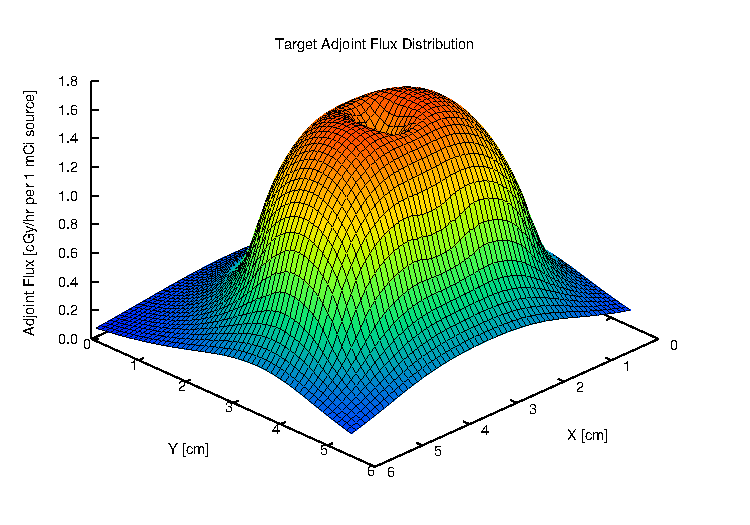
\includegraphics[width=2.5in]{figures/Target_adjoint_flux-midplane.pdf}
  \end{textblock}

   \begin{textblock}{20}(65,50)
    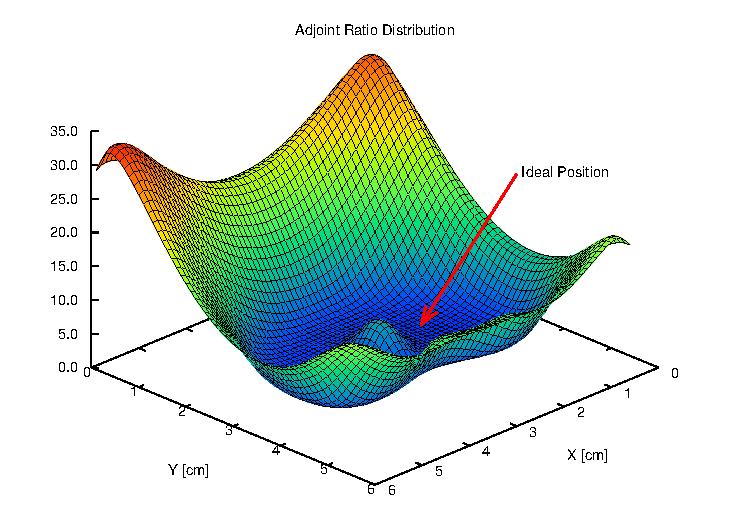
\includegraphics[width=2.5in]{figures/adjoint_ratio-slice5.pdf}
  \end{textblock}

\end{frame}

%%----------------------------------------------------------------------------%%
\begin{frame}{Detector design}
  
  \begin{textblock}{120}(4,15)
    \begin{itemize}
      \item The adjoint flux can allow for the spectral performance of a 
        detector to be predicted for an arbitrary source distribution.
      \item This data allows the detector design to be optimized before it is
        constructed, which is important for detectors with rare materials 
        (e.g. $He^3$ neutron detectors).
    \end{itemize}
  \end{textblock}

  \begin{textblock}{20}(2,50)
    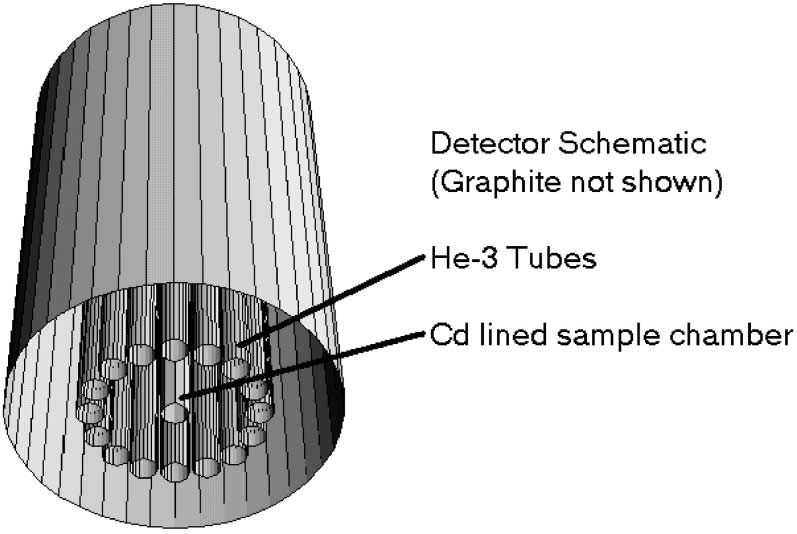
\includegraphics[width=2.5in]{figures/He3_detector.png}
  \end{textblock}

  \begin{textblock}{20}(70,49)
    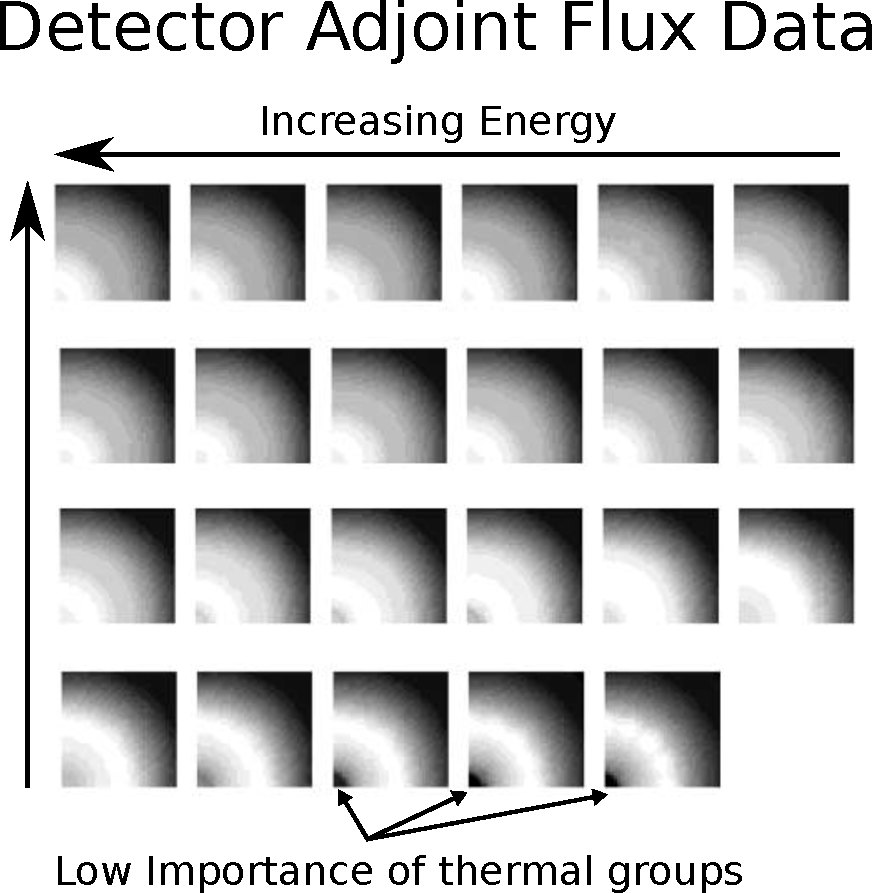
\includegraphics[width=1.8in]{figures/He3_detector_adjoint_data_modified.pdf}
  \end{textblock}

\end{frame}

%%----------------------------------------------------------------------------%%
\subsection{Monte Carlo codes available today}
%%----------------------------------------------------------------------------%%
\begin{frame}{Continuous energy capabilities of popular codes}
  
  \begin{table}[ht]
    \centering
    \begin{tabular}{c c c c c }
      \hline\hline
      Code & $n$ & $\gamma$ &  $n^{\dagger}$ & $\gamma^{\dagger}$ \\ [0.5ex]
      \hline
      EGS4 & - & $\surd$ & - & - \\
      EGSnrc & - & $\surd$ & - & - \\
      ITS6 & - & $\surd$ & - & - \\
      PENELOPE & - & $\surd$ & - & - \\
      MORSE & - & - & - & - \\
      TART2005 & $\surd$ & $\surd$ & - & - \\
      MCNP5/6 & $\surd$ & $\surd$ & - & - \\
      MCNPX & $\surd$ & $\surd$ & - & - \\
      GEANT4 & $\surd$ & $\surd$ & - & $\surd$ \\
      MCBEND & $\surd$ & $\surd$ & $\surd$ & - \\ [1ex]
      \hline
      FACEMC & $\surd$ & $\surd$ & $\surd$ & $\surd$ \\ [1ex]
      \hline
    \end{tabular}
  \end{table}

\begin{itemize}
  \item A lack of necessary adjoint cross section data is a major deterent to
    implementing the adjoint process on a continouous energy scale.
\end{itemize}
  
\end{frame}

%%----------------------------------------------------------------------------%%
\section{The Monte Carlo random walk process}
%%----------------------------------------------------------------------------%%
\subsection{General Monte Carlo theory}
%%----------------------------------------------------------------------------%%
\begin{frame}{Fredholm Integral Equations of the second kind (FIESKs)}

  \begin{beamerboxesrounded}{The FIESK}
    \begin{equation*}
      F(x) = S(x) + \lambda \int_a^b K(x,y) F(y)dy
      \label{eq:fredholm_int_eqn}
    \end{equation*}
  \end{beamerboxesrounded}
  
  \begin{itemize}
    \item The function $S(x)$ is a forcing function.
    \item The function $K(x,y)$ is the kernel of the integral equation
    \item $K(x,y)$ characterizes the transition from some initial state y to
      the state x.
    \item It is often written as $K(y \to x)$ to signify this interpretation.
  \end{itemize}
  
\end{frame}

%%----------------------------------------------------------------------------%%
\begin{frame}{The Volterra integral equation of the second kind}
  
  \begin{itemize}
    \item This equation is very similar to the FIESK except one limit of 
      integration is variable.
    \item This equation comes about whenever there is a preferred direction for 
      the independent variable (i.e. particle scattering kinematics)
    \item It can be written as a FIESK using a modified kernel
  \end{itemize}

  \begin{beamerboxesrounded}{The Volterra integral equation of the second kind}
    \begin{align}
      F(x) & = S(x) + \lambda \int_a^x K(y \to x) F(y) dy
      \nonumber \\
      & = S(x) + \lambda \int_a^b K^{'}(y \to x) F(y) dy \nonumber
    \end{align}
    \begin{equation*}
      K^{'}(y \to x) = 
      \begin{cases}
        K(y \to x) & \text{if }y < x \\
        0 & \text{if }y > x.
      \end{cases}
    \end{equation*}
  \end{beamerboxesrounded}

\end{frame}

%%----------------------------------------------------------------------------%%
\begin{frame}{Analytical solution method for a FIESK}

  \begin{beamerboxesrounded}{The method of successive approximations}
    \begin{align}
      f_0(x) & = S(x) \nonumber \\
      f_n(x) & = S(x) + \lambda \int_a^b K(y \to x)f_{n-1}(y)dy \nonumber \\
      & \quad \nonumber \\
      F(x) & = \lim_{n \to \infty} f_n(x) \nonumber \\
      & = S(x) + \lambda \int_a^b K(y \to x)S(y)dy + \nonumber \\
      & \quad \lambda^2 \int_a^b \int_a^b K(y \to x)K(y_1 \to y)S(y_1)dy_1dy +
      \nonumber \\
      & \quad \lambda^3 \int_a^b \int_a^b \int_a^b K(y \to x)K(y_1 \to y)
      K(y_2 \to y_1)S(y_2)dy_2dy_1dy + \nonumber \\
      & \quad \cdots \nonumber
    \end{align}
  \end{beamerboxesrounded}

\end{frame}

%%----------------------------------------------------------------------------%%
\begin{frame}{Numerical solution method for a FIESK}

  \begin{beamerboxesrounded}{The Monte Carlo random walk process}
    \begin{equation*}
      \text{Random Walk: }
      \begin{cases}
        p^1(x) & = p(x_1 = x) \\
        p(y \to x) & = p(x_{n+1} = x | x_n = y, k > n)  \\
        p(x) & = p(k = n | x_n = x).
      \end{cases}
      \label{eq:mc_random_walk_pdfs}
    \end{equation*}
  \end{beamerboxesrounded}

  \begin{itemize}
    \item $p^1(x)$ characterizes the probability that the first event of a
      random walk occurs in state $x$.
    \item $p(y \to x)$ characterizes the probability of a transition from an
      initial state $y$ to a new state $x$.
    \item $p(x)$ represents the probability of termination in a state $x$.
    \item The above probability distribution functions (PDFs) must have
      the following properties:
      \medskip
      \begin{enumerate}
        \item $p^1(x) \geq 0$ \newline
          $\int_{\Gamma} p^1(x)dx = 1$
        \medskip
        \item $p(y \to x) \geq 0$ \newline
          $\int_{\Gamma} p(y \to x)dx = q(y) = 1 - p(y)$.
      \end{enumerate}
  \end{itemize}

\end{frame}

%%----------------------------------------------------------------------------%%
\begin{frame}{Proof that the Monte Carlo method recovers the solution}

  \begin{itemize}
    \item First define the event density as the expected value of the number
      density of events that happen in state $x$:
      \begin{align}
        P(x) = 1 \cdot &P^1(x) + 1 \cdot P^2(x) + \ldots 
        = \sum_{n=1}^{\infty} P^n(x) \nonumber \\
        P^1(x) & = p^1(x) \nonumber \\
        P^n(x) & = \int_{\Gamma} p(y \to x) P^{n-1}(y)dy. \nonumber
      \end{align}
    \item Using the event density and the Monte Carlo method, the solution
      to a FIESK is recovered:
      \begin{align}
        P(x) & = \sum_{n=1}^{\infty} P^n(x) \nonumber
        = p^1(x) + \int_{\Gamma} p(y \to x) \sum_{n=2}^{\infty} P^{n-1}(y)dy 
        \nonumber\\
        & = p^1(x) + \int_{\Gamma} p(y \to x) P(y)dy \nonumber.
      \end{align}
  \end{itemize}

\end{frame}

%%----------------------------------------------------------------------------%%
\subsection{The Monte Carlo random walk process for radiation transport}
%%----------------------------------------------------------------------------%%
\begin{frame}{The transport equation}

\begin{equation*}
  \begin{split}
    \frac{1}{v}&\frac{\partial \varphi(\vec{r},E,\hat{\Omega},t)}{\partial t} +
    \hat{\Omega} \cdot \vec{\bigtriangledown} \varphi(\vec{r},E,\hat{\Omega},t)
    + \Sigma_T(\vec{r},E) \varphi(\vec{r},E,\hat{\Omega},t) = \\
    & \quad S(\vec{r},E,\hat{\Omega},t) +
    \int\int \Sigma_T(\vec{r},E^{'} \to E,\hat{\Omega^{'}} \to \hat{\Omega})
    \varphi(\vec{r},E^{'},\hat{\Omega^{'}},t) dE^{'}d\hat{\Omega^{'}} \nonumber
  \end{split}
\end{equation*}

  \begin{itemize}
    \item The transport equation describes the expected behavior of particles
      in a medium.
    \item This equation must be converted to a FIESK to derive a Monte Carlo
      random walk process.
    \item First define the emission density $\chi(\vec{r},E,\hat{\Omega})$, 
      which is the expected density of particles exiting a collision or the 
      source, as
      \newline
      \begin{align}
        \chi(\vec{r},E,\hat{\Omega}) = S(\vec{r},E,\hat{\Omega}) +
        \int\int &\Sigma_T(\vec{r},E^{'} \to E,\hat{\Omega}^{'} \to \hat{\Omega})
        \nonumber \\
        & \cdot \varphi(\vec{r},E^{'},\hat{\Omega}^{'}) dE^{'}d\hat{\Omega}^{'}.
        \nonumber
      \end{align}
  \end{itemize}

\end{frame}

%%----------------------------------------------------------------------------%%
\begin{frame}{Converting the transport equation to an integral form}

  \begin{itemize}
    \item The method of characteristics will be used to convert the 
      transport equation to an integral form: \newline
      \begin{equation*}
        \vec{r}^{'} = \vec{r} - R\hat{\Omega}.
        \label{eq:characteristic}
      \end{equation*}
    \item A directional derivative along the characteristic can be determined:
      \newline
      \begin{align}
        \frac{d}{dR} & = \frac{dx^{'}}{dR}\frac{\partial}{\partial x} +
        \frac{dy^{'}}{dR}\frac{\partial}{\partial y} +
        \frac{dz^{'}}{dR}\frac{\partial}{\partial z} \nonumber \\
        & = -\Omega_x \frac{\partial}{\partial x} -
        \Omega_y \frac{\partial}{\partial y} -
        \Omega_z \frac{\partial}{\partial z} \nonumber \\
        & = -\hat{\Omega} \cdot \vec{\bigtriangledown}. \nonumber
      \end{align}
    \item The transport equation becomes
      \begin{equation*}
        -\frac{d}{dR}\varphi(\vec{r}^{'},E,\hat{\Omega}) + \Sigma_T(\vec{r}^{'},E)
        \varphi(\vec{r}^{'},E,\hat{\Omega}) =
        \chi(\vec{r}^{'},E,\hat{\Omega}).
        \label{eq:transport_ode}
      \end{equation*}
  \end{itemize}

\end{frame}

%%----------------------------------------------------------------------------%%
\begin{frame}{The transport equation in integral form}

  \begin{itemize}
    \item Using the following integrating factor, the transport equation can
      be converted to an integral form: \newline
      \begin{equation*}
        \exp{\left[-\int_0^R \Sigma_T(\vec{r}-R^{'}\hat{\Omega},E)dR^{'} \right]}.
      \end{equation*}
    \item By integrating the equation from 0 to $\infty$ and assuming that the
      flux goes to zero as $R$ goes to $\infty$, the integral equation is
      obtained:
  \end{itemize}

  \begin{align}
    \varphi(\vec{r},E,\hat{\Omega}) & = 
    \int_0^{\infty} \chi(\vec{r} - R\hat{\Omega},E,\hat{\Omega})
    \exp{\left[-\int_0^R \Sigma_T(\vec{r}-R^{'}\hat{\Omega},E)dR^{'} \right]} 
    dR \nonumber \\
    & = \int \chi(\vec{r}^{'},E,\hat{\Omega}) 
    \tau(\vec{r}^{'},\vec{r},E,\hat{\Omega}) dV^{'}. \nonumber
  \end{align}

  \medskip

  \begin{equation*}
    \tau(\vec{r}^{'},\vec{r},E,\hat{\Omega})= 
    \exp{\left[-\int_0^{|\vec{r} - \vec{r}^{'}|} 
        \Sigma_T(\vec{r}-R^{'}\hat{\Omega},E)dR^{'} \right]} 
    \frac{\delta \left(\hat{\Omega} - \left[\frac{\vec{r} - \vec{r}^{'}}
        {|\vec{r} - \vec{r}^{'}|}\right]\right)}
         {|\vec{r} - \vec{r}^{'}|^2}
  \end{equation*}

\end{frame}

%%----------------------------------------------------------------------------%%
\begin{frame}{The emission density FIESK}

  \begin{itemize}
    \item To construct the emission density FIESK, the integral transport 
      equation will be substituted into the equation for the emission density:
  \end{itemize}
  \begin{align}
    \chi(\vec{r},E,\hat{\Omega}) & = S(\vec{r},E,\hat{\Omega}) +
    \int\int \Sigma_T(\vec{r},E^{'} \to E, \hat{\Omega}^{'} \to \hat{\Omega})
    \nonumber \\
    & \qquad \qquad \qquad \qquad \cdot
    \int \chi(\vec{r}^{'},E',\hat{\Omega}^{'})
    \tau(\vec{r}^{'},\vec{r},E^{'},\hat{\Omega}^{'})
    dV^{'}dE^{'}d\hat{\Omega}^{'} \nonumber \\
    & = S(\vec{r},E,\hat{\Omega}) + \int\int\int
    K(\vec{r}^{'} \to \vec{r}, E^{'} \to E, \hat{\Omega}^{'} \to \hat{\Omega})
    \nonumber \\
    & \qquad \qquad \qquad \qquad \qquad \cdot
    \chi(\vec{r}^{'},E',\hat{\Omega}^{'}) dV^{'}dE^{'}d\hat{\Omega}^{'}.
    \nonumber
  \end{align}

  \begin{itemize}
    \item The kernel of the emission density FIESK is
      \begin{align}
        K(y \to x) & = K(\vec{r}^{'} \to \vec{r}, E^{'} \to E, 
        \hat{\Omega}^{'} \to \hat{\Omega}) \nonumber \\
        & = \Sigma_T(\vec{r},E^{'} \to E, \hat{\Omega}^{'} \to \hat{\Omega})
        \tau(\vec{r}^{'},\vec{r},E^{'},\hat{\Omega}^{'}). \nonumber
      \end{align}
    \item This kernel can be simplified by introducing two new kernels.
  \end{itemize}

\end{frame}

%%----------------------------------------------------------------------------%%
\begin{frame}{The transport kernel}

  \begin{align}
    T(\vec{r}^{'} \to \vec{r},E,\hat{\Omega}) & = \Sigma_T(\vec{r},E)
    \tau(\vec{r}^{'},\vec{r},E,\hat{\Omega}) \nonumber \\
    & = \Sigma_T(\vec{r},E)
    \exp{\left[-\int_0^{|\vec{r} - \vec{r}^{'}|} 
        \Sigma_T(\vec{r}-R^{'}\hat{\Omega},E)dR^{'} \right]} \nonumber \\
    & \qquad \qquad \qquad \qquad \cdot
    \frac{\delta \left(\hat{\Omega} - \left[\frac{\vec{r} - \vec{r}^{'}}
        {|\vec{r} - \vec{r}^{'}|}\right]\right)}
         {|\vec{r} - \vec{r}^{'}|^2} \nonumber
  \end{align}

  \begin{itemize}
    \item This kernel describes the movement of particles through space.
    \item It is normalized to unity and can thus be used as a PDF for sampling
      new particle positions.
    \item The quantity $T(\vec{r}^{'} \to \vec{r},E,\hat{\Omega})dV$ can be 
      interpreted as the probability that a particle at $\vec{r}^{'}$ with 
      energy $E$ and direction $\hat{\Omega}$ will have its next collision in 
      volume element $dV$ at $\vec{r}$.
    \item Due to the factor $\Sigma_T(\vec{r},E)$, a new position $\vec{r}$ will
      never be sampled in a vacuum.
  \end{itemize}

\end{frame}

%%----------------------------------------------------------------------------%%
\begin{frame}{The collision kernel}

  \begin{equation*}
    C(\vec{r},E^{'} \to E, \hat{\Omega}^{'} \to \hat{\Omega}) =
    \frac{\Sigma_T(\vec{r},E^{'} \to E,\hat{\Omega}^{'} \to \hat{\Omega})}
         {\Sigma_T(\vec{r},E^{'})}
  \end{equation*}

  \begin{itemize}
    \item This kernel describes the movement of particles through energy
      and direction.
    \item Upon expansion, a procedure for sampling a new energy and direction
      from this kernel becomes clear:
  \end{itemize}

  \begin{align}
    C(\vec{r},&E^{'} \to E, \hat{\Omega}^{'} \to \hat{\Omega}) =
    \sum_j \frac{\Sigma_j(\vec{r},E^{'})c_i(\vec{r},E^{'})
      f_i(\vec{r},E^{'} \to E,\hat{\Omega}^{'} \to \hat{\Omega})}
        {\Sigma_T(\vec{r},E^{'})} \nonumber \\
      & = \sum_A \frac{\Sigma_A(\vec{r},E^{'})}{\Sigma_T(\vec{r},E^{'})}
        \sum_j \frac{\sigma_{A,j}(E^{'})}{\sigma_A(E^{'})} c_{A,j}(E^{'})
        p_{A,j}(E^{'} \to E,\hat{\Omega}^{'} \to \hat{\Omega}) \nonumber
  \end{align}

\end{frame}

%%----------------------------------------------------------------------------%%
\begin{frame}{The emission density FIESK revisited}

  \begin{itemize}
    \item Using the transport kernel and the collision kernel, the state
      transition kernel for the emission density FIESK can be simplified:
  \end{itemize}

  \begin{align}
    K(y \to x) & = K(\vec{r}^{'} \to \vec{r}, E^{'} \to E, 
    \hat{\Omega}^{'} \to \hat{\Omega}) \nonumber \\
    & = \Sigma_T(\vec{r},E^{'} \to E, \hat{\Omega}^{'} \to \hat{\Omega})
    \tau(\vec{r}^{'},\vec{r},E^{'},\hat{\Omega}^{'}) \nonumber \\
    & = \left[
      \frac{\Sigma_T(\vec{r},E^{'} \to E, \hat{\Omega}^{'} \to \hat{\Omega})}
    {\Sigma_T(\vec{r},E^{'})} \right]\left[\Sigma_T(\vec{r},E^{'}) 
    \tau(\vec{r}^{'},\vec{r},E^{'},\hat{\Omega}^{'})\right] \nonumber \\
    & = C(\vec{r},E^{'} \to E,\hat{\Omega}^{'} \to \hat{\Omega})
    T(\vec{r}^{'} \to \vec{r},E^{'},\hat{\Omega}^{'}) \nonumber
  \end{align}

  \begin{itemize}
    \item Sampling a new state from the state transition kernel $K(y \to x)$
      is now straightforward.
  \end{itemize}

\end{frame}

%%----------------------------------------------------------------------------%%
\begin{frame}{The collision density FIESK}    

  \begin{itemize}
    \item The collision density $\psi(\vec{r},E,\hat{\Omega})$ is the expected 
      density of particles entering a collision.
    \item It is related to the emission density by
      \begin{equation*}
        \psi(\vec{r},E,\hat{\Omega}) = \int 
        T(\vec{r}^{'} \to \vec{r},E,\hat{\Omega})
        \chi(\vec{r}^{'},E,\hat{\Omega})dV^{'}.
      \end{equation*}
    \item The collision density FIESK is therefore
  \end{itemize}
  \begin{align}
    \psi(\vec{r},E,\hat{\Omega}) & = \int S(\vec{r}^{'},E,\hat{\Omega})
    T(\vec{r}^{'} \to \vec{r},E,\hat{\Omega}) dV^{'} + \nonumber \\ 
    & \quad \int\int\int
    L(\vec{r}^{'} \to \vec{r},E^{'} \to E,\hat{\Omega}^{'} \to \hat{\Omega}) 
    \psi(\vec{r}^{'},E^{'},\hat{\Omega}^{'}) dE^{'}d\hat{\Omega}^{'}dV^{'}.
    \nonumber
  \end{align}
  \begin{itemize}
    \item The state transition kernel for this FIESK is
      \begin{align}
        L(y \to x) & = 
        L(\vec{r}^{'} \to \vec{r},E^{'} \to E,\hat{\Omega}^{'} \to \hat{\Omega}) 
        \nonumber \\
        & = T(\vec{r}^{'} \to \vec{r},E,\hat{\Omega})
        C(\vec{r}^{'},E^{'} \to E,\hat{\Omega}^{'} \to \hat{\Omega}). \nonumber
      \end{align}
  \end{itemize}
  
\end{frame}

%%----------------------------------------------------------------------------%%
\begin{frame}{The Monte Carlo process for radiation transport}

  \begin{itemize}
    \item The following PDFs govern the Monte Carlo random walk process
      for the emission density and collision density:
  \end{itemize}

  \begin{align}
    \chi(x)\text{ Random Walk:} &
    \begin{cases}
      p^1(x) & = \frac{S(x)}{\int_{\Gamma} S(x)dx} \\
      p(y \to x) &  = K(y \to x) \\
      p(x) & = 1 - \overline{P}_{NA}(x),
    \end{cases} \nonumber \\ \medskip
    \psi(x)\text{ Random Walk:} &
    \begin{cases}
      p^1(x) & = \frac{S_c(x)}{\int_{\Gamma} S_c(x)dx} \\
      p(y \to x) & = L(y \to x) \\
      p(x) & = 1 - P_{NA}(x).
    \end{cases}
    \nonumber
  \end{align}

  \begin{itemize}
    \item $P_{NA}(x) = \frac{\Sigma_s(\vec{r},E^{'})}{\Sigma_T(\vec{r},E^{'})}$ is
      the non-absorption or survival probability.
    \item $\overline{P}_{NA}(x)$ is an average survival probability along the 
      line from $\vec{r}^{'}$ to $\vec{r}$.
    \item $S_c(x)$ is the first collided source.
    \item Both processes can be combined into a single process.
  \end{itemize}
    
\end{frame}

%%----------------------------------------------------------------------------%%
\begin{frame}{The combined Monte Carlo process}

  \begin{textblock}{120}(4,15)
    \begin{itemize}
      \item The state transition kernels for the emission density and the
        collision density only differ in the ordering of the transport and
        collision kernels.
      \item They can therefore be estimated during the same random walk process.
    \end{itemize}
  \end{textblock}

  \begin{textblock}{20}(50,45)
    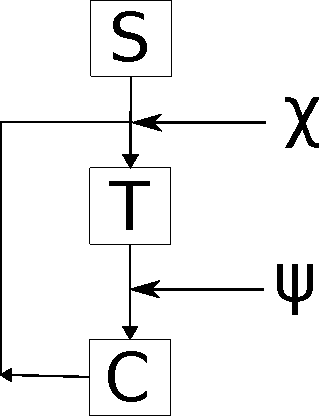
\includegraphics[width=1.25in]{../document/chapters/random_walk_process_derivation/random_walk_process.pdf}
  \end{textblock}

  %% \begin{textblock}{20}(80,50)
  %%   \begin{align}
  %%     R & = \langle r \text{ } \varphi \rangle \nonumber \\
  %%     & = \langle r_{\psi} \text{ } \psi \rangle \nonumber \\
  %%     & = \langle r_{\chi} \text{ } \chi \rangle \nonumber
  %%   \end{align}
  %% \end{textblock}

\end{frame}

%%----------------------------------------------------------------------------%%
\subsection{The Monte Carlo random walk process for adjoint radiation transport}
%%----------------------------------------------------------------------------%%
\begin{frame}{Derivation of the adjoint transport equation}

  \begin{itemize}
    \item An adjoint operator is defined by the following relationship:
      \begin{equation*}
        \langle \varphi^{\dagger}H_B \cdot \varphi \rangle = 
        \langle \varphi H_B^{\dagger} \cdot \varphi^{\dagger} \rangle.
      \end{equation*}
    \item The transport equation can be written in an operator form:
      \begin{equation*}
        H_B \cdot \varphi(\vec{r},E,\hat{\Omega}) = S(\vec{r},E,\hat{\Omega}).
      \end{equation*}
    \item A material response can be calculated using the flux and a material
      response function $r(\vec{r},E,\hat{\Omega})$:
      \begin{equation*}
        R = \langle \varphi r \rangle.
      \end{equation*}
    \item If $H_B^{\dagger} \cdot \varphi^{\dagger}$ is set equal to the response 
      function, the material response becomes
      \begin{align}
        R & = \langle \varphi r \rangle 
        = \langle \varphi H_B^{\dagger} \cdot \varphi^{\dagger} \rangle \nonumber \\
        & = \langle \varphi^{\dagger}H_B \cdot \varphi \rangle
        = \langle \varphi^{\dagger} S \rangle \nonumber.
      \end{align}
  \end{itemize}

\end{frame}

%%----------------------------------------------------------------------------%%
\begin{frame}{The adjoint transport equation}

  \begin{itemize}
    \item Using the transport equation in operator form and the definition
      of the adjoint operator, the adjoint transport equation can be derived.
    \item The adjoint transport equation is 
  \end{itemize}
  \begin{equation*}
    \begin{split}
      -\hat{\Omega} &\cdot \vec{\bigtriangledown} 
      \varphi^{\dagger}(\vec{r},E,\hat{\Omega})
      + \Sigma_T(\vec{r},E) \varphi^{\dagger}(\vec{r},E,\hat{\Omega}) = \\
      & \quad r(\vec{r},E,\hat{\Omega}) +
      \int\int \Sigma_T(\vec{r},E \to E^{'},\hat{\Omega} \to \hat{\Omega}^{'})
      \varphi^{\dagger}(\vec{r},E^{'},\hat{\Omega}^{'}) dE^{'}d\hat{\Omega}^{'}.
    \end{split}
  \end{equation*}

  \begin{itemize}
    \item The adjoint emission denisty will be defined as
  \end{itemize}
  \begin{equation*}
    \theta^{\dagger}(\vec{r},E,\hat{\Omega}) = r(\vec{r},E,\hat{\Omega}) +
    \int\int \Sigma_T(\vec{r},E \to E^{'},\hat{\Omega} \to \hat{\Omega}^{'})
    \varphi^{\dagger}(\vec{r},E^{'},\hat{\Omega}^{'}) dE^{'}d\hat{\Omega}^{'}.
  \end{equation*}

  \begin{itemize}
    \item The simplified adjoint transport equation is
  \end{itemize}
  \begin{equation*}
    -\hat{\Omega} \cdot \vec{\bigtriangledown} 
      \varphi^{\dagger}(\vec{r},E,\hat{\Omega})
      + \Sigma_T(\vec{r},E) \varphi^{\dagger}(\vec{r},E,\hat{\Omega}) =
      \theta^{\dagger}(\vec{r},E,\hat{\Omega}).
  \end{equation*} 
      
\end{frame}

%%----------------------------------------------------------------------------%%
\begin{frame}{The adjoint transport equation in integral form}

  \begin{itemize}
    \item Using a very similar process to the one used for the transport 
      equation the adjoint transport equation can be converted to an
      integral form:
  \end{itemize}
  \begin{align}
    \varphi^{\dagger}(\vec{r},E,\hat{\Omega}) & = 
    \int_0^{\infty} \theta^{\dagger}(\vec{r} + R\hat{\Omega},E,\hat{\Omega})
    exp\left[-\int_0^R \Sigma_T(\vec{r}+R^{'}\hat{\Omega},E)dR^{'} \right] dR
    \nonumber \\
    & = \int \theta^{\dagger}(\vec{r}^{'},E,\hat{\Omega}) 
    \tau^{\dagger}(\vec{r}^{'},\vec{r},E,\hat{\Omega}) dV^{'}. \nonumber
  \end{align}

  \begin{equation*}
    \tau^{\dagger}(\vec{r}^{'},\vec{r},E,\hat{\Omega}) = 
    \exp{\left[-\int_0^{|\vec{r}^{'} - \vec{r}|} 
        \Sigma_T(\vec{r}+R^{'}\hat{\Omega},E)dR^{'} \right]}
    \frac{\delta \left(\Omega - \left[\frac{\vec{r}^{'} - \vec{r}}
        {|\vec{r}^{'} - \vec{r}|}\right]\right)}
         {|\vec{r}^{'} - \vec{r}|^2}.
  \end{equation*}

\end{frame}

%%----------------------------------------------------------------------------%%
\begin{frame}{The adjoint emission density FIESK}

  \begin{itemize}
    \item To construct the adjoint emission density FIESK, the integral 
      adjoint transport equation will be substituted into the equation for
      the adjoint emission density:
  \end{itemize}
  \begin{align}
    \theta^{\dagger}(\vec{r},E,\hat{\Omega}) & = r(\vec{r},E,\hat{\Omega}) +
    \int\int \Sigma_T(\vec{r},E \to E^{'},\hat{\Omega} \to \hat{\Omega}^{'})
    \nonumber \\
    & \qquad \qquad \qquad \qquad \cdot
    \int \theta^{\dagger}(\vec{r}^{'},E^{'},\hat{\Omega}^{'}) 
    \tau^{\dagger}(\vec{r}^{'},\vec{r},E^{'},\hat{\Omega}^{'}) 
    dV^{'} dE^{'} d\hat{\Omega}^{'} \nonumber \\
    & = r(\vec{r},E,\hat{\Omega}) +
    \int\int\int M^{\dagger}(\vec{r}^{'} \to \vec{r},E^{'} \to E,
        \hat{\Omega}^{'} \to \hat{\Omega}) \nonumber \\
         & \qquad \qquad \qquad \qquad \qquad \cdot
         \theta^{\dagger}(\vec{r}^{'},E^{'},\hat{\Omega}^{'}) 
         dV^{'} dE^{'} d\hat{\Omega}^{'}. \nonumber
  \end{align}

  \begin{itemize}
    \item The kernel of the adjoint emission density FIESK is
      \begin{align}
        M^{\dagger}(y \to x) & = M^{\dagger}(\vec{r}^{'} \to \vec{r},E^{'} \to E,
        \hat{\Omega}^{'} \to \hat{\Omega}) \nonumber \\
        & = \Sigma_T(\vec{r},E \to E^{'},\hat{\Omega} \to \hat{\Omega}^{'})
        \tau^{\dagger}(\vec{r}^{'},\vec{r},E^{'},\hat{\Omega}^{'}) \nonumber
      \end{align}
    \item This kernel can be simplified by introducing two new kernels
  \end{itemize}

\end{frame}

%%----------------------------------------------------------------------------%%
\begin{frame}{The adjoint transport kernel}

  \begin{align}
    T^{\dagger}(\vec{r}^{'} \to \vec{r},E,\hat{\Omega}) & = 
    \Sigma_T(\vec{r},E) \tau^{\dagger}(\vec{r}^{'},\vec{r},E,\hat{\Omega})
    \nonumber \\
    & = \Sigma_T(\vec{r},E) \exp{\left[-\int_0^{|\vec{r}^{'} - \vec{r}|} 
        \Sigma_T(\vec{r}+R^{'}\hat{\Omega},E)dR^{'} \right]} \nonumber \\
    & \qquad \qquad \qquad \qquad \cdot
    \frac{\delta \left(\Omega - \left[\frac{\vec{r}^{'} - \vec{r}}
        {|\vec{r}^{'} - \vec{r}|}\right]\right)}
         {|\vec{r}^{'} - \vec{r}|^2} \nonumber
  \end{align}

  \begin{itemize}
    \item This kernel describes the movement of adjoint particles through space.
    \item It is normalized to unity and can thus be used as a PDF for sampling
      new particle positions.
    \item The quantity $T^{\dagger}(\vec{r}^{'} \to \vec{r},E,\hat{\Omega})dV$ can
      be interpreted as the probability that an adjoint particle at 
      $\vec{r}^{'}$ with energy $E$ and direction $\hat{\Omega}$ will have its 
      next collision in volume element $dV$ at $\vec{r}$.
  \end{itemize}

\end{frame}

%%----------------------------------------------------------------------------%%
\begin{frame}{The adjoint collision kernel}

  \begin{align}
    C^{\dagger}(\vec{r},E^{'} \to E,\hat{\Omega}^{'} \to \hat{\Omega}) & = 
    \frac{\Sigma_T(\vec{r},E \to E^{'},\hat{\Omega} \to \hat{\Omega}^{'})}
         {\int\int \Sigma_T(\vec{r},E \to E^{'},\hat{\Omega} \to \hat{\Omega}^{'})
           dE d\hat{\Omega}} \nonumber \\
         & = \frac{\Sigma_T(\vec{r},E \to E^{'},\hat{\Omega} \to \hat{\Omega}^{'})}
         {\Sigma^{\dagger}(\vec{r},E^{'})} \nonumber
  \end{align}

  \begin{itemize}
    \item This kernel describes the movement of adjoint particles through 
      energy and direction.
    \item The normalization factor for this kernel will be referred to simply
      as the total macroscopic adjoint cross section.
    \item To derive a sampling procedure for this kernel, it must be expanded
      into its constituent reactions.
  \end{itemize}

\end{frame}

%%----------------------------------------------------------------------------%%
\begin{frame}{The expanded adjoint collision kernel}
  
  \begin{align}
    C^{\dagger}(\vec{r},&E^{'} \to E,\hat{\Omega}^{'} \to \hat{\Omega}) =
    \frac{\Sigma_T(\vec{r},E \to E^{'},\hat{\Omega} \to \hat{\Omega}^{'})}
         {\Sigma^{\dagger}(\vec{r},E^{'})} \nonumber \\
         & = \sum_j 
         \frac{\Sigma_{j}(\vec{r},E)c_j(\vec{r},E)
           f_j(E \to E^{'},\hat{\Omega} \to \hat{\Omega}^{'})}
              {\Sigma^{\dagger}(\vec{r},E^{'})} \nonumber \\
              & = \sum_A \frac{\Sigma_A^{\dagger}(\vec{r},E^{'})}
              {\Sigma^{\dagger}(\vec{r},E^{'})}
              \sum_j \frac{\sigma_{A,j}^{\dagger}(E^{'})}{\sigma_A^{\dagger}(E^{'})}
              \frac{\sigma_{A,j}(E) c_{A,j}(E) 
                p_{A,j}(E \to E^{'},\hat{\Omega} \to \hat{\Omega}^{'})}
                   {\sigma_{A,j}^{\dagger}(E^{'})} \nonumber
  \end{align}

  \begin{itemize}
    \item Through expansion of this kernel, the definition of the adjoint
      cross section also becomes clear:
      \begin{equation*}
        \sigma_{A,j}^{\dagger}(E^{'}) = \int\int
        \sigma_{A,j}(E)c_{A,j}(E) 
        p_{A,j}(E \to E^{'},\hat{\Omega} \to \hat{\Omega}^{'}) dE d\hat{\Omega}
      \end{equation*}
      \begin{equation*}
        p_{A,j}^{\dagger}(E^{'} \to E,\hat{\Omega}^{'} \to \hat{\Omega}) = 
        \frac{\sigma_{A,j}(E)c_{A,j}(E) 
          p_{A,j}(E \to E^{'},\hat{\Omega} \to \hat{\Omega}^{'})}
             {\sigma_{A,j}^{\dagger}(E^{'})}
      \end{equation*}
  \end{itemize}
  
\end{frame}

%%----------------------------------------------------------------------------%%
\begin{frame}{The adjoint emission density FIESK revisited}
  
  \begin{itemize}
    \item Using the adjoint transport kernel and the adjoint collision kernel,
      the state transition kernel for the adjoint emission density FIESK 
      can be simplified:
  \end{itemize}

  \begin{align}
    M^{\dagger}(y \to x) & = M^{\dagger}(\vec{r}^{'} \to \vec{r},E^{'} \to E,
    \hat{\Omega}^{'} \to \hat{\Omega}) \nonumber \\
    & = \Sigma_T(\vec{r},E \to E^{'},\hat{\Omega} \to \hat{\Omega}^{'})
    \tau^{\dagger}(\vec{r}^{'},\vec{r},E^{'},\hat{\Omega}^{'}) \nonumber \\
    & = \left[
      \frac{\Sigma_T(\vec{r},E \to E^{'},\hat{\Omega} \to \hat{\Omega}^{'})}
           {\Sigma^{\dagger}(\vec{r},E^{'})}\right]
    \left[\frac{\Sigma^{\dagger}(\vec{r},E^{'})}{\Sigma_T(\vec{r},E^{'})}\right]
    \nonumber \\
    & \qquad \cdot \left[\Sigma_T(\vec{r},E^{'})
    \tau^{\dagger}(\vec{r}^{'},\vec{r},E^{'},\hat{\Omega}^{'})\right] \nonumber \\
    & = C^{\dagger}(\vec{r},E^{'} \to E,\hat{\Omega}^{'} \to \hat{\Omega})
    P^{\dagger}(\vec{r},E^{'})
    T^{\dagger}(\vec{r}^{'} \to \vec{r},E^{'},\hat{\Omega}^{'}). \nonumber
  \end{align}

  \begin{itemize}
    \item This kernel also contains a factor $P^{\dagger}(\vec{r},E^{'})$ called 
      the adjoint weight factor.
    \item This factor is bounded in the interval (0,$\infty$).
  \end{itemize}

\end{frame}

%%----------------------------------------------------------------------------%%
\begin{frame}{The adjoint collision density FIESK}

  \begin{itemize}
    \item The adjoint collision density $\xi^{\dagger}(\vec{r},E,\hat{\Omega})$
      is the expected density of adjoint particles entering a collision.
    \item It is related to the adjoint emission density by
      \begin{equation*}
        \xi^{\dagger}(\vec{r},E,\hat{\Omega}) =
        \int T^{\dagger}(\vec{r}^{'} \to \vec{r},E,\hat{\Omega})
        \theta^{\dagger}(\vec{r}^{'},E,\hat{\Omega}) dV^{'}.
      \end{equation*}
    \item The adjoint collision density FIESK is therefore
  \end{itemize}
  \begin{align}
    \xi^{\dagger}(\vec{r},E,\hat{\Omega}) & = \int r(\vec{r}^{'},E,\hat{\Omega})
    T^{\dagger}(\vec{r}^{'} \to \vec{r},E,\hat{\Omega}) dV^{'} + \nonumber \\
    &\quad \int\int\int N^{\dagger}(\vec{r}^{'} \to \vec{r},E^{'} \to E,
    \hat{\Omega}^{'} \to \hat{\Omega}) 
    \xi^{\dagger}(\vec{r}^{'},E^{'},\hat{\Omega}^{'})
    dE^{'}d\hat{\Omega}^{'}dV^{'}. \nonumber
  \end{align}
  
  \begin{itemize}
    \item The state transition kernel for this FIESK is
  \end{itemize}
  \begin{align}
    N^{\dagger}(y \to x) & =
    N^{\dagger}(\vec{r}^{'} \to \vec{r},E^{'} \to E,\hat{\Omega}^{'} \to \hat{\Omega})
    \nonumber \\
    & = T^{\dagger}(\vec{r}^{'} \to \vec{r},E,\hat{\Omega})
    C^{\dagger}(\vec{r}^{'},E^{'} \to E,\hat{\Omega}^{'} \to \hat{\Omega})
    P^{\dagger}(\vec{r}^{'},E^{'}). \nonumber
  \end{align}
  
\end{frame}

%%----------------------------------------------------------------------------%%
\begin{frame}{The Monte Carlo random walk process for adjoint radiation transport}
  \begin{itemize}
    \item The following PDFs govern the Monte Carlo random walk process for
      the adjoint emission density and the adjoint collision density:
  \end{itemize}
  \begin{align}
    \theta^{\dagger}(x)\text{ Random Walk:}&
    \begin{cases}
      p^1(x) & = \frac{a(x)}{\int_{\Gamma} a(x)dx} \\
      p(y \to x) & = \frac{M^{\dagger}(y \to x)}{\overline{P}^{\dagger}(y)} \\
      p(x) & = 0
    \end{cases} \nonumber \\
    \xi^{\dagger}(x)\text{ Random Walk:}&
    \begin{cases}
      p^1(x) & = \frac{S_c^{\dagger}(x)}{\int_{\gamma} S_c^{\dagger}(x)dx} \\
      p(y \to x) & = \frac{N^{\dagger}(y \to x)}{P^{\dagger}(y)} \\
      p(x) & = 0.
    \end{cases} \nonumber
  \end{align}

  \begin{itemize}
    \item Due to the definition of the adjoint cross section, there is no
      absorption reaction for adjoint radiation.
    \item Russian roulette must be used to end random walks.
    \item Both processes can be combined into a single process.
  \end{itemize}

\end{frame}

%%----------------------------------------------------------------------------%%
\begin{frame}{The combined Monte Carlo adjoint process}

  \begin{textblock}{120}(4,15)
    \begin{itemize}
      \item The state transition kernels for the emission density and the 
        collision density only differ in the ordering of the adjoint transport
        kernel, adjoint collision kernel, and adjoint weight factor.
      \item They can therefore be estimated during the same random walk process.
    \end{itemize}
  \end{textblock}

  \begin{textblock}{20}(50,45)
    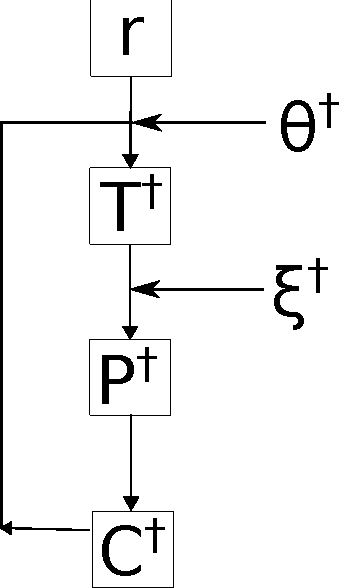
\includegraphics[width=1.0in]{figures/adjoint_random_walk_process.pdf}
  \end{textblock}

\end{frame}

%%----------------------------------------------------------------------------%%
\section{Adjoint Photon Cross Sections}
%%----------------------------------------------------------------------------%%
\subsection{Adjoint photon incoherent scattering}
%%----------------------------------------------------------------------------%%
\begin{frame}{Developing the adjoint incoherent scattering cross section}
  
  \begin{itemize}
    \item To conduct adjoint incoherent scattering, the cross section for 
      this interaction must be derived:
  \end{itemize}
  \begin{align}
    p_{i.s}^{\dagger}(E^{'} \to E, \hat{\Omega}^{'} \to \hat{\Omega}) & =
    \frac{\sigma_{i.s.}(E)c_{i.s.}(E)
      p_{i.s.}(E \to E^{'},\hat{\Omega} \to \hat{\Omega}^{'})}
         {\sigma_{i.s.}^{\dagger}(E^{'})} \nonumber \\
         \sigma_{i.s.}^{\dagger}(E^{'})
         p_{i.s}^{\dagger}(E^{'} \to E, \hat{\Omega}^{'} \to \hat{\Omega}) & = 
         \sigma_{i.s.}(E)p_{i.s.}(E \to E^{'},\hat{\Omega} \to \hat{\Omega}^{'})
         \nonumber \\
         \sigma_{i.s}^{\dagger}(E^{'} \to E, \hat{\Omega}^{'} \to \hat{\Omega}) & = 
         \sigma_{i.s.}(E \to E^{'},\hat{\Omega} \to \hat{\Omega}^{'}) \nonumber
  \end{align}

  \begin{itemize}
    \item Both the forward and adjoint cross sections are only dependent on the 
      angle between the initial and final directions:
  \end{itemize}
  
  \begin{align}
    \sigma_{i.s}^{\dagger}(E^{'} \to E, \hat{\Omega}^{'} \cdot \hat{\Omega}) & = 
    \sigma_{i.s.}(E \to E^{'},\hat{\Omega} \cdot \hat{\Omega}^{'}) \nonumber \\
    \sigma_{i.s}^{\dagger}(E^{'} \to E, \mu) & = 
    \sigma_{i.s.}(E \to E^{'}, \mu). \nonumber
  \end{align}

\end{frame}

%%----------------------------------------------------------------------------%%
\begin{frame}{The adjoint incoherent scattering cross section}

  \begin{itemize}
    \item The double differential incoherent scattering cross section is
  \end{itemize}
  \begin{align}
    \sigma_{i.s.}(E^{'} \to E, \mu) & = 
    \frac{d\sigma_{i.s.}(E^{'},E,\mu,Z)}{dEd\mu} \nonumber \\
    & =  \frac{\pi r_e^2}{m_ec^2 \alpha^{'2}}
    \left[\frac{\alpha}{\alpha^{'}} + \frac{\alpha^{'}}{\alpha} - 
      1 + \mu^2\right] S\left(y(\alpha^{'},\mu),Z\right) \nonumber \\
    & \qquad \qquad \qquad \cdot \delta\left(\mu - \left[1-\frac{1}{\alpha} + 
      \frac{1}{\alpha^{'}}\right]\right). \nonumber
  \end{align}

  \begin{itemize}
    \item The adjoint double differential incoherent scattering cross section
      is therefore
  \end{itemize}
   \begin{align}
    \sigma_{i.s.}^{\dagger}(E^{'} \to E, \mu)  & =  
    \frac{\pi r_e^2}{m_ec^2 \alpha^{2}}
    \left[\frac{\alpha^{'}}{\alpha} + \frac{\alpha}{\alpha^{'}} - 
      1 + \mu^2\right] S\Big(y(\alpha,\mu),Z\Big) \nonumber \\
    & \qquad \qquad \qquad \cdot \delta\left(\mu - \left[1-\frac{1}{\alpha^{'}} 
      + \frac{1}{\alpha}\right]\right). \nonumber
  \end{align}

\end{frame}

%%----------------------------------------------------------------------------%%
\begin{frame}{The integrated adjoint incoherent scattering cross section}

  \begin{textblock}{120}(4,15)
    \begin{itemize}
      \item The scattering kinematics of the adjoint interaction have an
        interesting property:
        \begin{equation*}
          E = \frac{E^{'}}{1-\alpha^{'}(1-\mu)}
        \end{equation*}
      \item There is a discontinuity when $\mu = 1 - \frac{1}{\alpha^{'}}$,
        which results in an unbound integrated cross section.
      \item A max problem energy must be set to bound the integrated 
        cross section.
    \end{itemize}
  \end{textblock}

  \begin{textblock}{20}(37,53)
    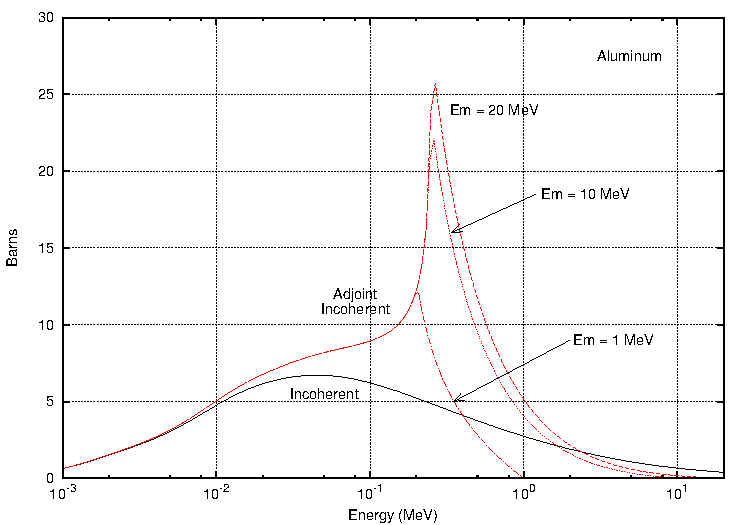
\includegraphics[width=2.4in]{figures/adjoint_and_forward_incoherent_cross_section-13.pdf}
  \end{textblock}
  
\end{frame}

%%----------------------------------------------------------------------------%%
\subsection{Adjoint photon coherent scattering}
%%----------------------------------------------------------------------------%%
\begin{frame}{The adjoint coherent scattering cross section}

  \begin{itemize}
    \item To conduct adjoint coherent scattering, the cross section for this
      interaction must be derived.
    \item The forward and adjoint cross sections are only dependent on the angle
      between the initial and final directions.
    \item In addition, the energy of the photon does not change in a forward
      coherent scatter:
  \end{itemize}
  \begin{align}
  \sigma_{c.s.}^{\dagger}(E^{'} \to E, \hat{\Omega}^{'} \to \hat{\Omega}) & =
  \sigma_{c.s.}(E \to E^{'},\hat{\Omega} \to \hat{\Omega}^{'}) \nonumber \\
  \sigma_{c.s.}^{\dagger}(E^{'}, \hat{\Omega}^{'} \cdot \hat{\Omega}) & = 
  \sigma_{c.s.}(E^{'},\hat{\Omega} \cdot \hat{\Omega}^{'}) \nonumber \\
  \sigma_{c.s.}^{\dagger}(E^{'}, \mu) & = \sigma_{c.s.}(E^{'}, \mu). \nonumber
\end{align}

  \begin{itemize}
    \item Both the forward and adjoint differential coherent scattering cross
      section are therefore the same:
      \begin{align}
        \frac{d\sigma_{c.s.}(\alpha^{'},\mu,Z)}{d\mu} & = 
        \frac{d\sigma_{c.s.}^{\dagger}(\alpha^{'},\mu,Z)}{d\mu} \nonumber \\
        & = \pi r_e^2 (1 + \mu^2)F^2(y,Z). \nonumber
      \end{align}
  \end{itemize}

\end{frame}

%%----------------------------------------------------------------------------%%
\subsection{Adjoint photon pair production}
%%----------------------------------------------------------------------------%%
\begin{frame}{Developing the adjoint pair production cross section}

  \begin{itemize}
    \item To conduct adjoint pair production, the cross section for this
      interaction must be derived.
    \item As with all other photon cross sections, these cross sections are
      only depenedent on the angle between the initial and final directions:
  \end{itemize}
  \begin{align}
    \sigma_{p.p.}^{\dagger}(E^{'} \to E, \hat{\Omega}^{'} \to \hat{\Omega}) & = 
    \sigma_{p.p.}(E \to E^{'}, \hat{\Omega} \to \hat{\Omega}^{'}) \nonumber \\
    \sigma_{p.p.}^{\dagger}(E^{'} \to E,\mu) & =  
    \sigma_{p.p.}(E \to E^{'},\mu) \nonumber
    %% \frac{d^2\sigma_{p.p.}^{\dagger}(E^{'},E,Z)}{dEd\mu} & = 
    %% \frac{d^2\sigma_{p.p.}^{\dagger}(E,E^{'},Z)}{dE^{'}d\mu}
  \end{align}

  \begin{itemize}
    \item The simplified double differential pair production cross section is
  \end{itemize}
  \begin{align}
    \sigma_{p.p.}(E^{'} \to E,\mu) & = \frac{d^2\sigma_{p.p.}(E^{'},Z)}{dEd\mu} 
    \nonumber \\
    & = \frac{2 [\sigma_{p.p.}(E^{'},Z) + \sigma_{t.p.}(E^{'},Z)] 
      \delta(E - m_ec^2)}{2}. \nonumber
  \end{align}
  
\end{frame}

%%----------------------------------------------------------------------------%%
\begin{frame}{The adjoint pair production cross section}

  \begin{itemize}
    \item The adjoint pair production cross section is
  \end{itemize}
  \begin{align}
    \sigma_{p.p.}^{\dagger}(E^{'} \to E,\mu) & = 
    \frac{d^2\sigma_{p.p.}^{\dagger}(E^{'},E,Z)}{dEd\mu} \nonumber \\
    & = \frac{2\left[\sigma_{p.p.}(E,Z)+\sigma_{t.p.}(E,Z)\right]
      \delta(E^{'}-m_ec^2)}{2}. \nonumber
  \end{align}

  \begin{itemize}
    \item The adjoint double differential pair production cross section will be
      zero unless the initial energy of the adjoint photon is equal to $m_ec^2$.
    \item A modification to the adjoint Monte Carlo random walk process must
      be made for adjoint photons to model adjoint pair production.
    \item The modification is rather complicated and will not be discussed
      further in this presentation. 
  \end{itemize}

\end{frame}  

%%----------------------------------------------------------------------------%%
\begin{frame}{The photoelectric effect}

  \begin{itemize}
    \item The photoelectric effect occurs when a photon of energy E is absorbed
      by a target atom.
    \item An electron will be ejected leaving an electron shell vacancy.
    \item Atomic relaxation will occur to fill the vacancy, which has the
      potential to release x-rays.
    \item These x-rays can be important for certain problems (e.g. brachytherapy
      seed characterization).
    \item The adjoint process cannot currently take these x-rays into account
      since there is not an equivalent adjoint reaction.
  \end{itemize}

\end{frame}

%%----------------------------------------------------------------------------%%
\subsection{The adjoint photon weight factor}
%%----------------------------------------------------------------------------%%
\begin{frame}{The adjoint photon weight factor}

  \begin{textblock}{120}(4,15)
    \begin{itemize}
      \item The adjoint weight factor is an important feature of the adjoint 
        process.
      \item Because it is bound to the interval (0,$\infty$) instead of (0,1) it
        can negatively effect the statistics of the random walks.
      \item Many test problems will need to be run to characterize the effect
        for adjoint photons.
    \end{itemize}
  \end{textblock}

  \begin{textblock}{20}(36,42)
    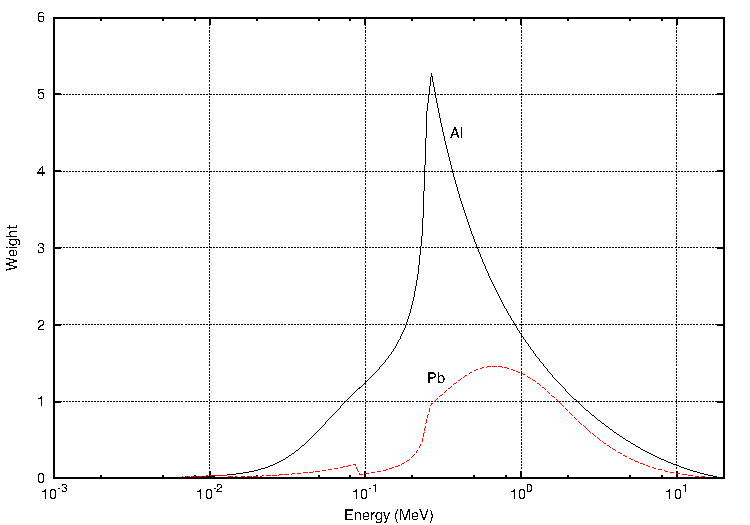
\includegraphics[width=3.0in]{../document/chapters/photon_interactions/adjoint_weight_factor.pdf}
  \end{textblock}
  
\end{frame}

%%----------------------------------------------------------------------------%%
\section{Forward-Adjoint Continuous Energy Monte Carlo (FACEMC)}
%%----------------------------------------------------------------------------%%
\subsection{Code overview}
%%----------------------------------------------------------------------------%%
\begin{frame}{FACEMC code requirements}

  \begin{itemize}
    \item The FACEMC code will be able to model photons and adjoint photons
      in the energy range of 1 keV to 20 MeV.
    \item The FACEMC code will also be able to model neutrons and adjoint
      neutrons in the energy range of $10^{-5}$ eV to 20 MeV.
    \item The direct accelerated geometry (DAG) package will primarily used
      for spatial domain modeling.
    \item The main variance reduction techniques that will be available are
      Russian roulette, splitting, and weight windows.
    \item The code will be able to run in parallel using domain replication
      only.
  \end{itemize}

\end{frame}

%%----------------------------------------------------------------------------%%
\begin{frame}{Major Components of FACEMC}
  
  \begin{textblock}{20}(20,15)
    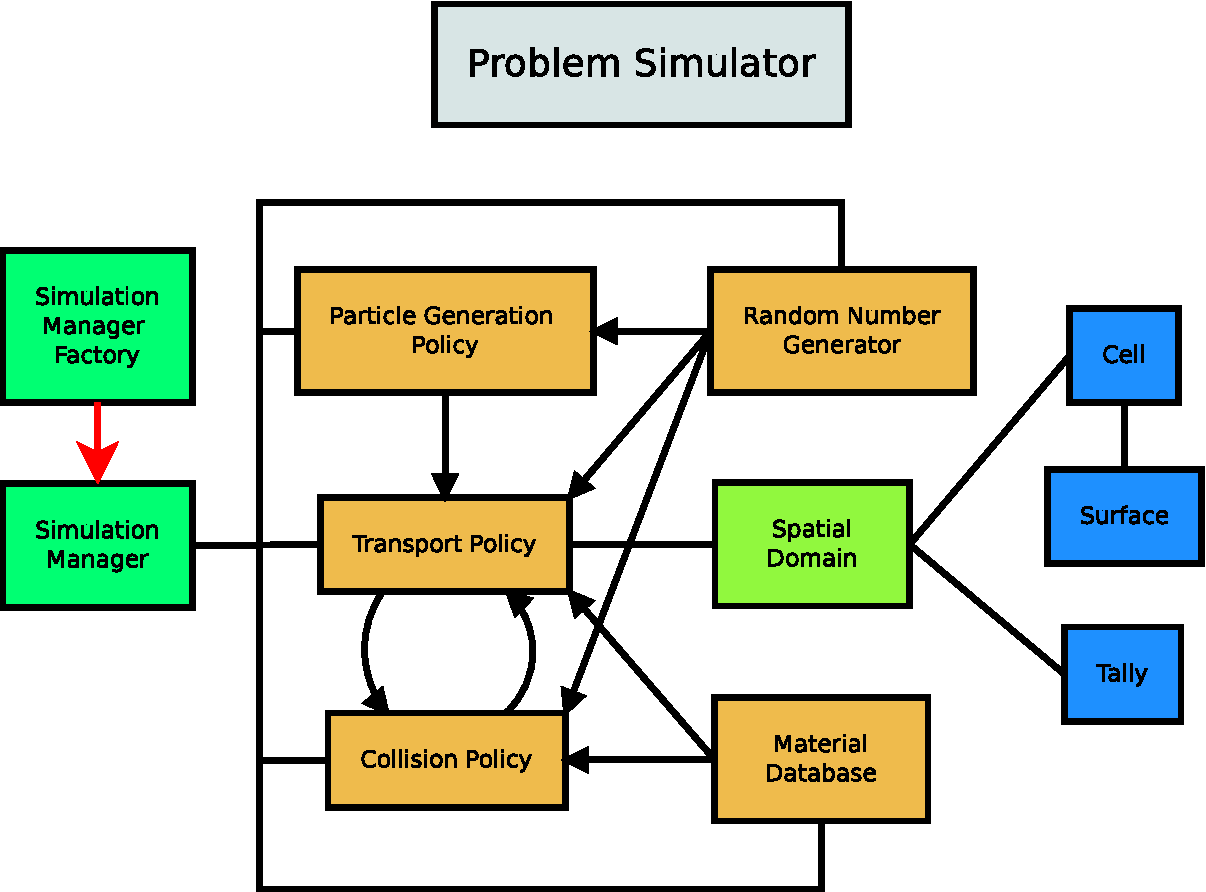
\includegraphics[width=3.5in]{../document/chapters/code_overview/Problem_Simulator.pdf}
  \end{textblock}

  \begin{textblock}{120}(4,85)
    \begin{itemize}
      \item FACEMC version 1.0 is currently complete.
    \end{itemize}
  \end{textblock}

\end{frame}

%%----------------------------------------------------------------------------%%
\subsection{Validation Plan}
%%----------------------------------------------------------------------------%%
\begin{frame}{FACEMC validation plan}

  \begin{itemize}
    \item The following validation plan has been created to ensure that FACEMC
      functions properly:
      \begin{enumerate}
        \item Calculation of benchmark test problems for photons and neutrons
        \item Code-to-code comparisons of integral quantities and photon or 
          neutron spectra against other Monte Carlo codes that have been 
          previously validated
        \item Comparison of integral quantities and spectra from forward and 
          reverse simulations
      \end{enumerate}
    \item Each step will be elaborated upon.
  \end{itemize}

\end{frame}

%%----------------------------------------------------------------------------%%
\begin{frame}{FACEMC validation plan step 1}

  \begin{textblock}{120}(4,15)
    \begin{itemize}
      \item The same benchmark problem that was used to validate GEANT4 photon
        simulations will be used with FACEMC.
      \item In this problem, photon mass attenuation coefficients and partial
        interaction coefficients will be calculated and compared to NIST values
    \end{itemize}
  \end{textblock}
  
  \begin{textblock}{20}(30,43)
    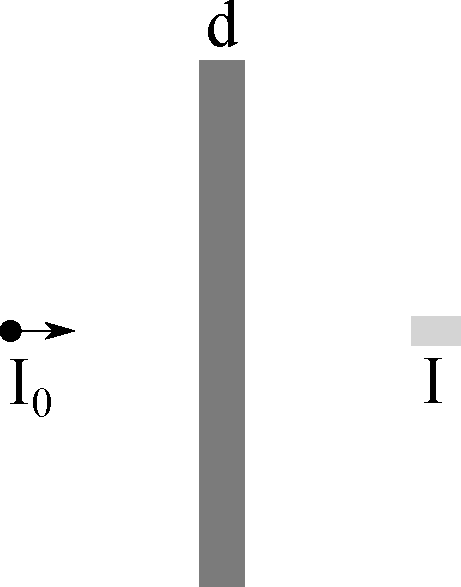
\includegraphics[width=1.0in]{../document/chapters/code_overview/photon_benchmark_problem.pdf}
  \end{textblock}

  \begin{textblock}{20}(65,52)
    \begin{equation*}
      \left(\frac{\mu}{\rho}\right) = -\frac{1}{\rho d}
      \ln{\left(\frac{\text{I}}{\text{I}_0}\right)}
    \end{equation*}
  \end{textblock}

  \begin{textblock}{120}(4,80)
    \begin{itemize}
      \item For neutrons, several experiments from the Shielding Integral
        Benchmark Archive Database (SINBAD) will be modeled.
    \end{itemize}
  \end{textblock}

\end{frame}

%%----------------------------------------------------------------------------%%
\begin{frame}{FACEMC validation plan step 2}
  
  \begin{textblock}{120}(4,15)
    \begin{itemize}
      \item A code-to-code comparison problem has been created to test
        FACEMC agains codes that have already been validated:
    \end{itemize}
  \end{textblock}

  \begin{textblock}{20}(43,27)
    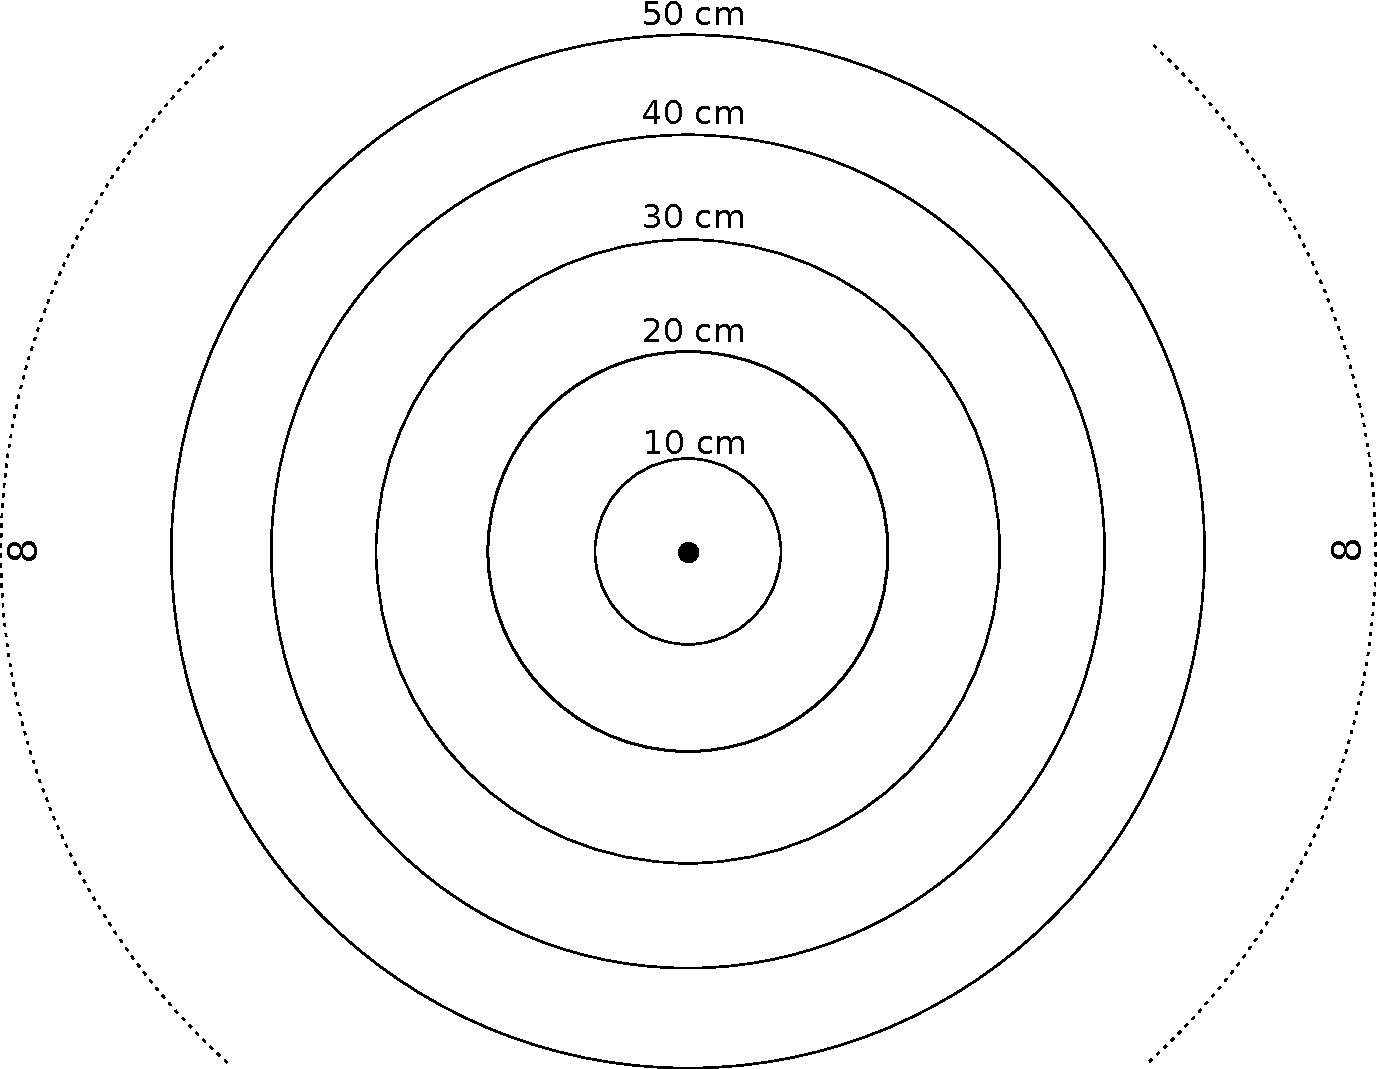
\includegraphics[width=1.7in]{figures/code_comparison_problem.pdf}
  \end{textblock}

  \begin{textblock}{120}(4,62)
    \begin{itemize}
      \item For photons, an isotropic point source with two
        discrete energies will be modeled.
      \item For neutrons, an isotropic point source with a
        fission spectrum will be modeled.
      \item PENELOPE, MCNP5 and TART2005 will be the codes
        that are tested against.
    \end{itemize}
  \end{textblock}

\end{frame}

%%----------------------------------------------------------------------------%%
\begin{frame}{FACEMC validation plan step 3}

  \begin{itemize}
    \item The third step of the validation plan will focus
      on comparisons between forward and adjoin calculations
      using FACEMC only.
    \item The problem from step 2 will be used.
    \item Due to unique symmetry in that problem, the adjoint problem can be 
      constructed identically to the forward problem.
    \item A proof of this symmetry is lengthy and will not be shown in this
      presentation.
  \end{itemize}    

\end{frame}

%%----------------------------------------------------------------------------%%
\begin{frame}{Preliminary validation of FACEMC: AMOS comparison}

   \begin{textblock}{120}(4,15)
    \begin{itemize}
      \item A comparison to the AMOS code was made using a simple model
        of an irradiation facility.
      \item A Cs-137 gamma source is located behind the tungsten alloy 
        collimator.
      \item The flux spectrum 50 cm from the center of the source on the
        axis of the source was calculated.
    \end{itemize}
  \end{textblock}

  \begin{textblock}{20}(43,50)
    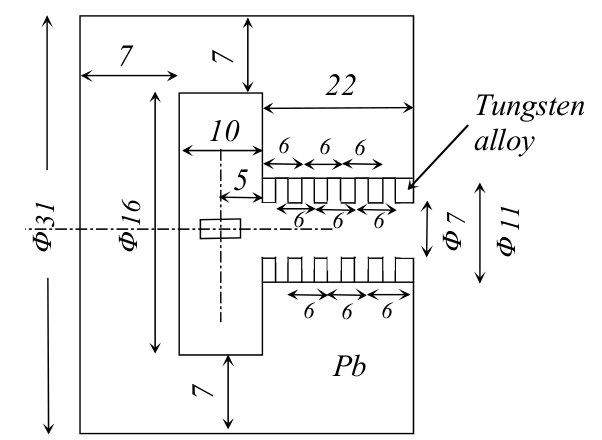
\includegraphics[width=2.3in]{figures/Irradiator_Facility.png}
  \end{textblock}

\end{frame}

%%----------------------------------------------------------------------------%%
\begin{frame}{AMOS comparison results}

  \begin{figure}[h!]
    \begin{center}
      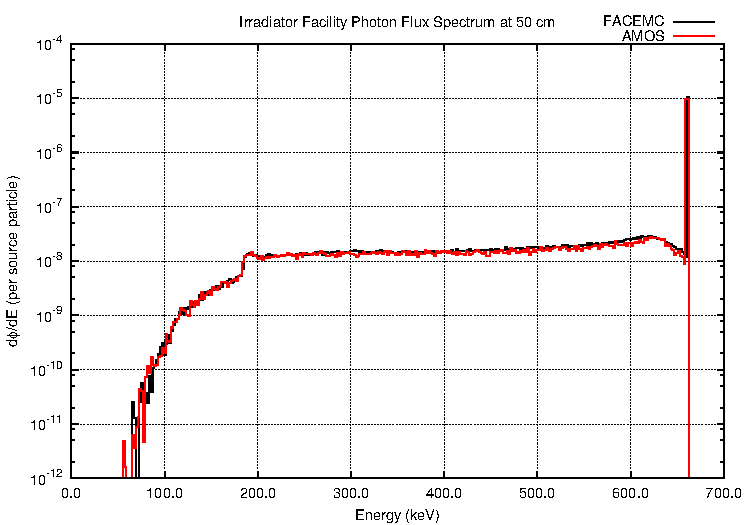
\includegraphics[width=4in]{figures/facemc_amos_irradiator_comp.pdf}
    \end{center}
  \end{figure}

\end{frame}

%%----------------------------------------------------------------------------%%
\begin{frame}{Preliminary validation of FACEMC: forward vs. adjoint}

   %%\begin{textblock}{120}(4,15)
    \begin{itemize}
      \item The problem from validation step 3 was used.
      \item \textbf{Source energies:} 661.66 keV, 321.0 keV
      \item \textbf{Material:} water
      \item \textbf{Number of histories:} $10^7$
    \end{itemize}
   %%\end{textblock}

    \begin{table}[ht]
      \centering
      \begin{tabular}{c c c c c c}
        \hline\hline
        Distance & Flux & Relative & Flux & Relative & \% Diff. \\ 
        (cm) & (for. mode) & Error & (adj. mode) & Error &  \\ [0.5ex]
        \hline
        10 & 1.5748e-3 & 0.0007 & 1.5788e-3 & 0.0014 & 0.25 \\
        20 & 4.1291e-4 & 0.0007 & 4.1491e-4 & 0.0018 & 0.48 \\
        30 & 1.4150e-4 & 0.0007 & 1.4235e-4 & 0.0022 & 0.60 \\
        40 & 5.2255e-5 & 0.0011 & 5.2322e-5 & 0.0027 & 0.13 \\
        50 & 1.9963e-5 & 0.0014 & 2.0030e-5 & 0.0033 & 0.34 \\ [1ex]
        \hline
      \end{tabular}
      \label{table:val_plan_s3_c0_flux_water}
    \end{table}   

\end{frame}

%%----------------------------------------------------------------------------%%
\begin{frame}{Forward vs. adjoint spectrum results}
  
  \begin{figure}[h!]
     \begin{center}
       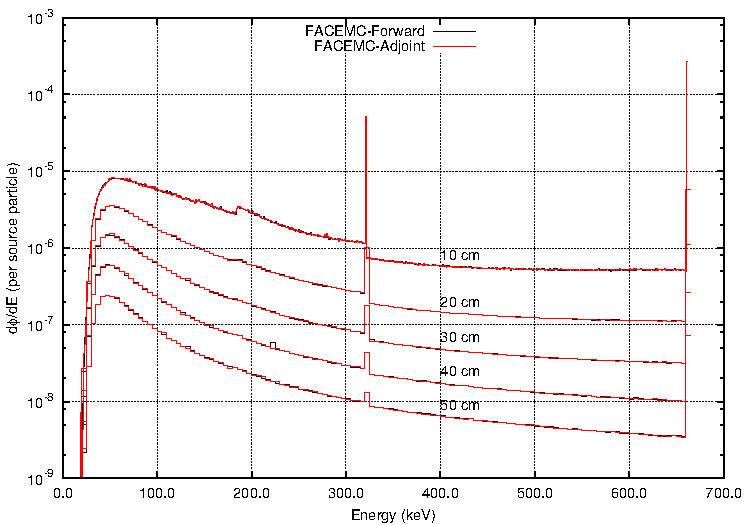
\includegraphics[width=4in]{../document/chapters/code_overview/photon_spectrum_validation_comparison.pdf}
     \end{center}
   \end{figure}

\end{frame}

%%----------------------------------------------------------------------------%%
\section{Future Work}
%%----------------------------------------------------------------------------%%
\begin{frame}{Future work on FACEMC}

  \begin{itemize}
    \item \textbf{Development work:} 
      \begin{enumerate}
        \item Solve the low energy x-ray emission problem for adjoint photons.
        \item Complete background work on neutron and adjoint neutron transport 
          cross sections and sampling techniques.
        \item Complete coding of the second version of all major FACEMC 
          components.
        \item Complete the computation of adjoint neutron cross sections and 
          storage in an HDF5 format library.
        \item Complete the FACEMC validation plan.
      \end{enumerate}
  \item \textbf{Challenge Problems:}
    \begin{enumerate}
      \item Calculate the adjoint data required for brachytherapy treatment 
        planning optimization using data from a patient.
      \item Calculate the adjoint data required for external beam treatment 
        planning using a standard phantom.
      \item Run a full scale shutdown dose calculation for a fusion device using
        the R2SA method.
      \item Run a shielding problem using the adjoint neutron transport 
        capabilities of FACEMC.
    \end{enumerate}
  \end{itemize}

\end{frame}

%%----------------------------------------------------------------------------%%

\end{document}

